\documentclass{beamer}
\usepackage{fancyvrb}

\usecolortheme{rose}
\usecolortheme{whale}
\usefonttheme{structurebold}
\setbeamercovered{again covered=\opaqueness<1->{50}}

\title[lh]{Domain-specific Static Analysis with ``Lighthouse''}
\author{Joseph Birr-Pixton}
\date{28th October 2009}

\begin{document}

\frame{\titlepage}

\frame
{
  \frametitle{Contents}

  \begin{enumerate}
    \item<1> Orientation.
    \item<2> Design and architecture.
    \item<3> Results from analysis of \texttt{nglibs} and \texttt{ntl}.
  \end{enumerate}
}

\frame
{
  \frametitle{Introduction}
  Definitions (my own):

  \begin{description}
    \item[General purpose SA] SA with respect to standard language features,
                              standard libraries, or common OS interfaces.
                              \textit{Examples: Coverity, Klocwork, Fortify, most compilers.}
    \item[Domain-specific SA] User-controlled SA of custom APIs.
                              \textit{Example: sparse.}
  \end{description}

  But:

  \begin{itemize}
  \item<2-> Most general purpose SA systems support customisation.
  \item<3-> A domain-specific SA system is a general purpose SA system with some difficult bits missing.
  \end{itemize}
}

\frame
{
  \frametitle{Orientation}

  ``Let's construct a useful domain-specific SA thing from bits we have lying around...''
}

\frame
{
  \frametitle{Design}

  \begin{itemize}
  \item<1-> We have a good, very well tested C/C++ parser.  \uncover<2->{It's called GCC.}
  \item<3-> We have a wide selection of languages available for writing SA rules.  \uncover<4->{`Programming' languages, if you will.}
  \item<5-> GCC is \emph{already} suitably integrated with whatever build system is used.
  \item<6-> Compile and SA in one step will almost always be quicker than separate compile and SA processes: let's abolish the difference.
  \end{itemize}
}

\frame
{
  \frametitle{Design}
  Aims:

  \begin{itemize}
  \item<1-> Let's write as little C as possible.
  \item<2-> Let's minimise the amount of stuff needing to be kept in sync with GCC's fluid
            internal APIs.
  \item<3-> Let's not require any specific language for writing rules.
  \end{itemize}
}

\frame
{
  \frametitle{Design}
  \begin{itemize}
    \item<1-> A shared object (written in a minimal amount of C) gets dynamically loaded into
              GCC, installs itself as a compilation pass and squirts detailed IR\footnote{intermediate representation}
              at a subprocess (`lh-pipe').
    \item<2-> Subprocess inherits GCC's \texttt{stdout}/\texttt{stderr} and produces arbitrary output.
    \item<3-> Non-zero subprocess exit causes GCC to fail in turn and end the build.
  \end{itemize}
}

\frame
{
  \frametitle{IR}

  \begin{itemize}
    \item<1-> Based on GIMPLE (GCC's internal IR).
     \item<2-> Only 4(!) essential statements:
     \begin{enumerate}
       \item<3->{Assignment (lhs = rhs, lhs = op rhs, lhs = rhs1 op rhs2)}
       \item<4->{Function call (lhs = func(args, ...))}
       \item<5->{Condition (if (expr) goto block1 else goto block2)}
       \item<6->{Switch (switch (expr) case val: goto block1; ...)}
    \end{enumerate}
    \item<7-> Encodes control flow graph.
    \item<8-> XML-based.
    \item<9-> Contains full source file for reporting purposes.
    \item<10-> Details of all referenced external types and functions.
    \item<11-> Actual alignment and size information for aggregate types.
  \end{itemize}
}

\begin{frame}[fragile]
  \frametitle{Example IR}

\footnotesize \begin{verbatim}
#include <stdio.h>

int main(void)
{
  printf("hello world!\n");
  return 0;
}
\end{verbatim}
\normalsize

Compiled with:

\footnotesize \begin{verbatim}
$ gcc -fplugin=lighthouse-client.so -o helloworld helloworld.c
\end{verbatim}
\normalsize

Produces (other than the desired executable)...
\end{frame}

\begin{frame}[fragile]
\tiny \begin{verbatim}
<lh-translation-unit client-version="0.1" filename="helloworld.c" language="C">
  <raw-source>#include &lt;stdio.h&gt;

int main(void)
{
  printf("hello world!\n");
  return 0;
}
</raw-source>
  <referenced-types>
  </referenced-types>
  <function-bodies>
    <function body-begin="4" body-end="7" location="helloworld.c:3" name="main">
      <returns>
        <integer name="int" precision="32" />
      </returns>
      <args>
      </args>
      <body entrypoint="2">
        <locals>
          <local location="helloworld.c:6:3">
            <binding id="2472" />
            <type alignment="32" size="32">
              <integer name="int" precision="32" />
            </type>
          </local>
        </locals>
\end{verbatim}
\end{frame}

\begin{frame}[fragile]
\tiny \begin{verbatim}
        <block id="2">
          <call location="helloworld.c:5:9">
            <function id="739" name="__builtin_puts" />
            <lhs>
              <void />
            </lhs>
            <args>
              <addr-of>
                <item-ref>
                  <array>
                    <constant>
                      <array id="1521">
                        <type>
                          <integer constant="1" name="char" precision="8" />
                        </type>
                        <domain>
                          <integer max="12" min="0" precision="32" />
                        </domain>
                      </array>
                      <string-literal>hello world!\x00</string-literal>
                    </constant>
                  </array>
                  <index>
                    <constant>
                      <integer name="int" precision="32" />
                      <integer-literal value="0" />
                    </constant>
                  </index>
                </item-ref>
              </addr-of>
            </args>
          </call>
\end{verbatim}
\end{frame}

\begin{frame}[fragile]
\tiny \begin{verbatim}
          <assign location="helloworld.c:6:3">
            <lhs>
              <bound id="2472" />
            </lhs>
            <rhs>
              <constant>
                <integer name="int" precision="32" />
                <integer-literal value="0" />
              </constant>
            </rhs>
          </assign>
          <return>
            <bound id="2472" />
          </return>
        </block>
      </body>
      <externals>
        <external location="&lt;built-in&gt;:0:0">
          <binding id="739" name="__builtin_puts" />
          <type alignment="8">
            <function attributes="nonnull">
              <return>
                <integer name="int" precision="32" />
              </return>
              <arguments>
                <addr-of>
                  <integer constant="1" name="char" precision="8" />
                </addr-of>
                <void />
              </arguments>
            </function>
          </type>
        </external>
      </externals>
    </function>
  </function-bodies>
</lh-translation-unit>
\end{verbatim}
\end{frame}

\frame
{
  \frametitle{Desired end architecture}

  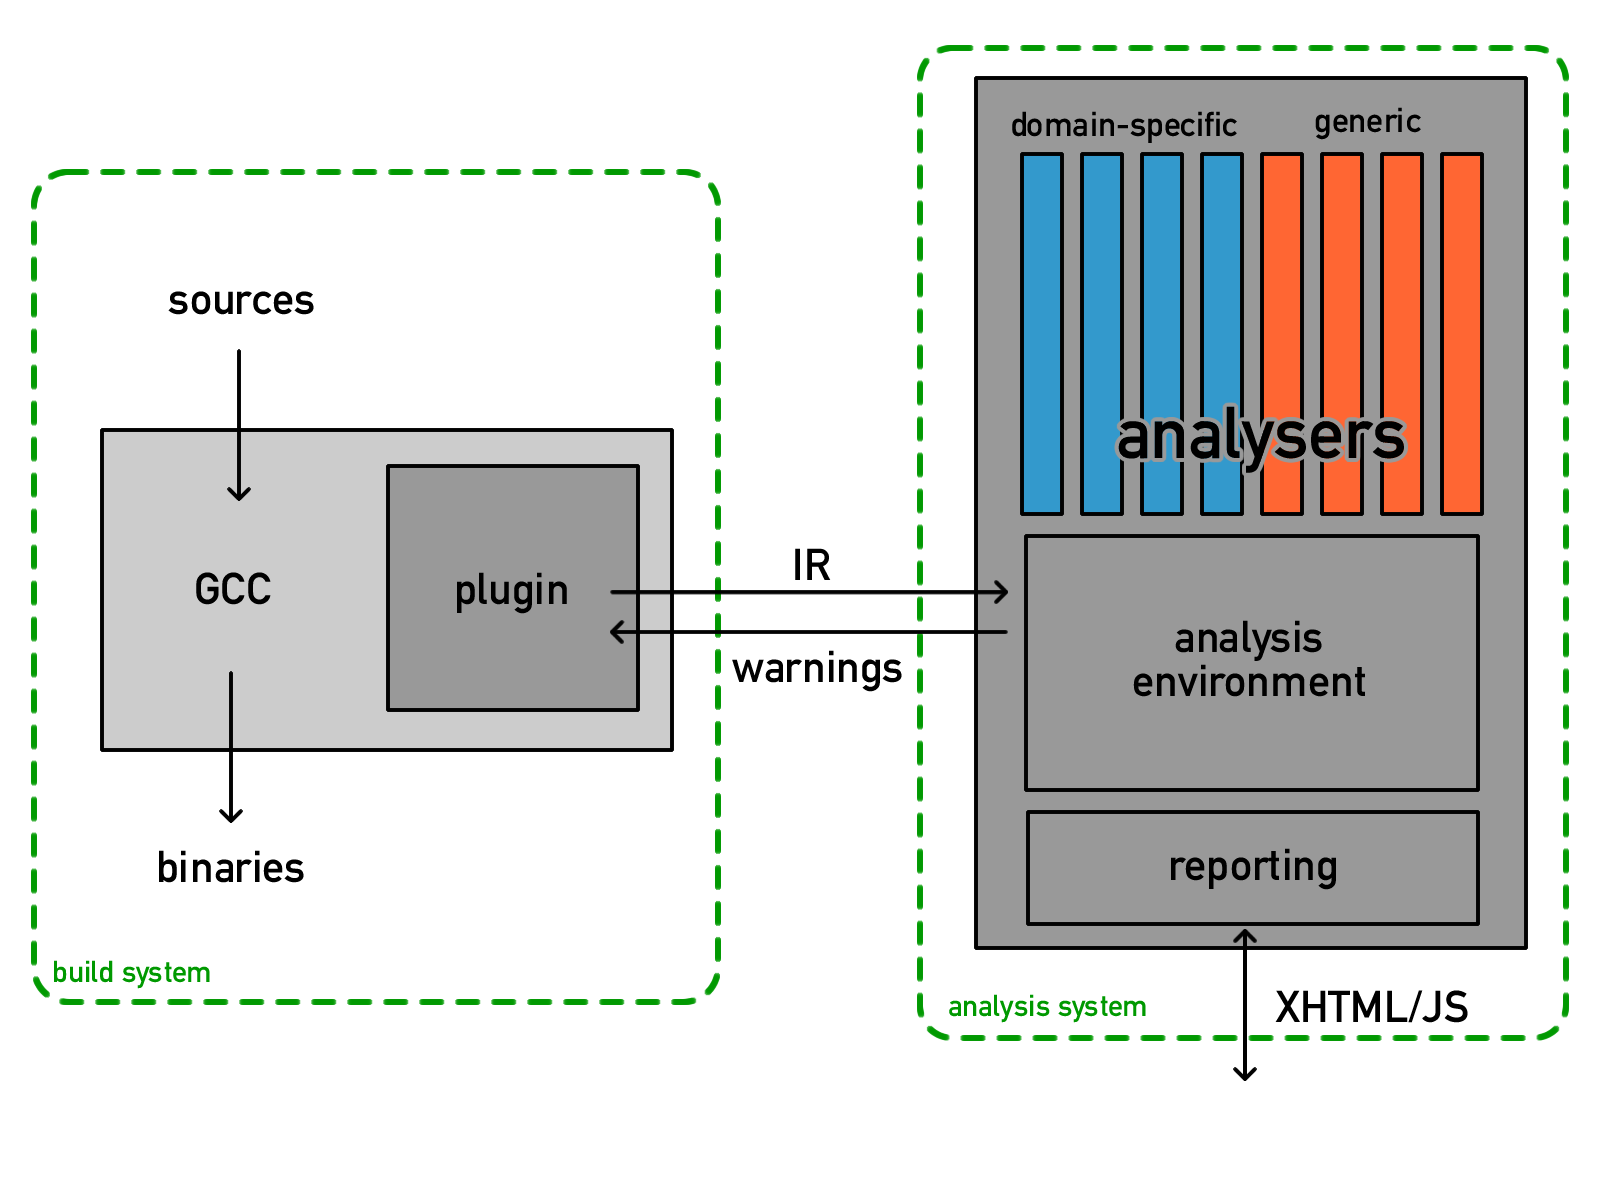
\includegraphics[width=1.0\textwidth]{arch.png}
}

\frame
{
  \frametitle{Current status}

  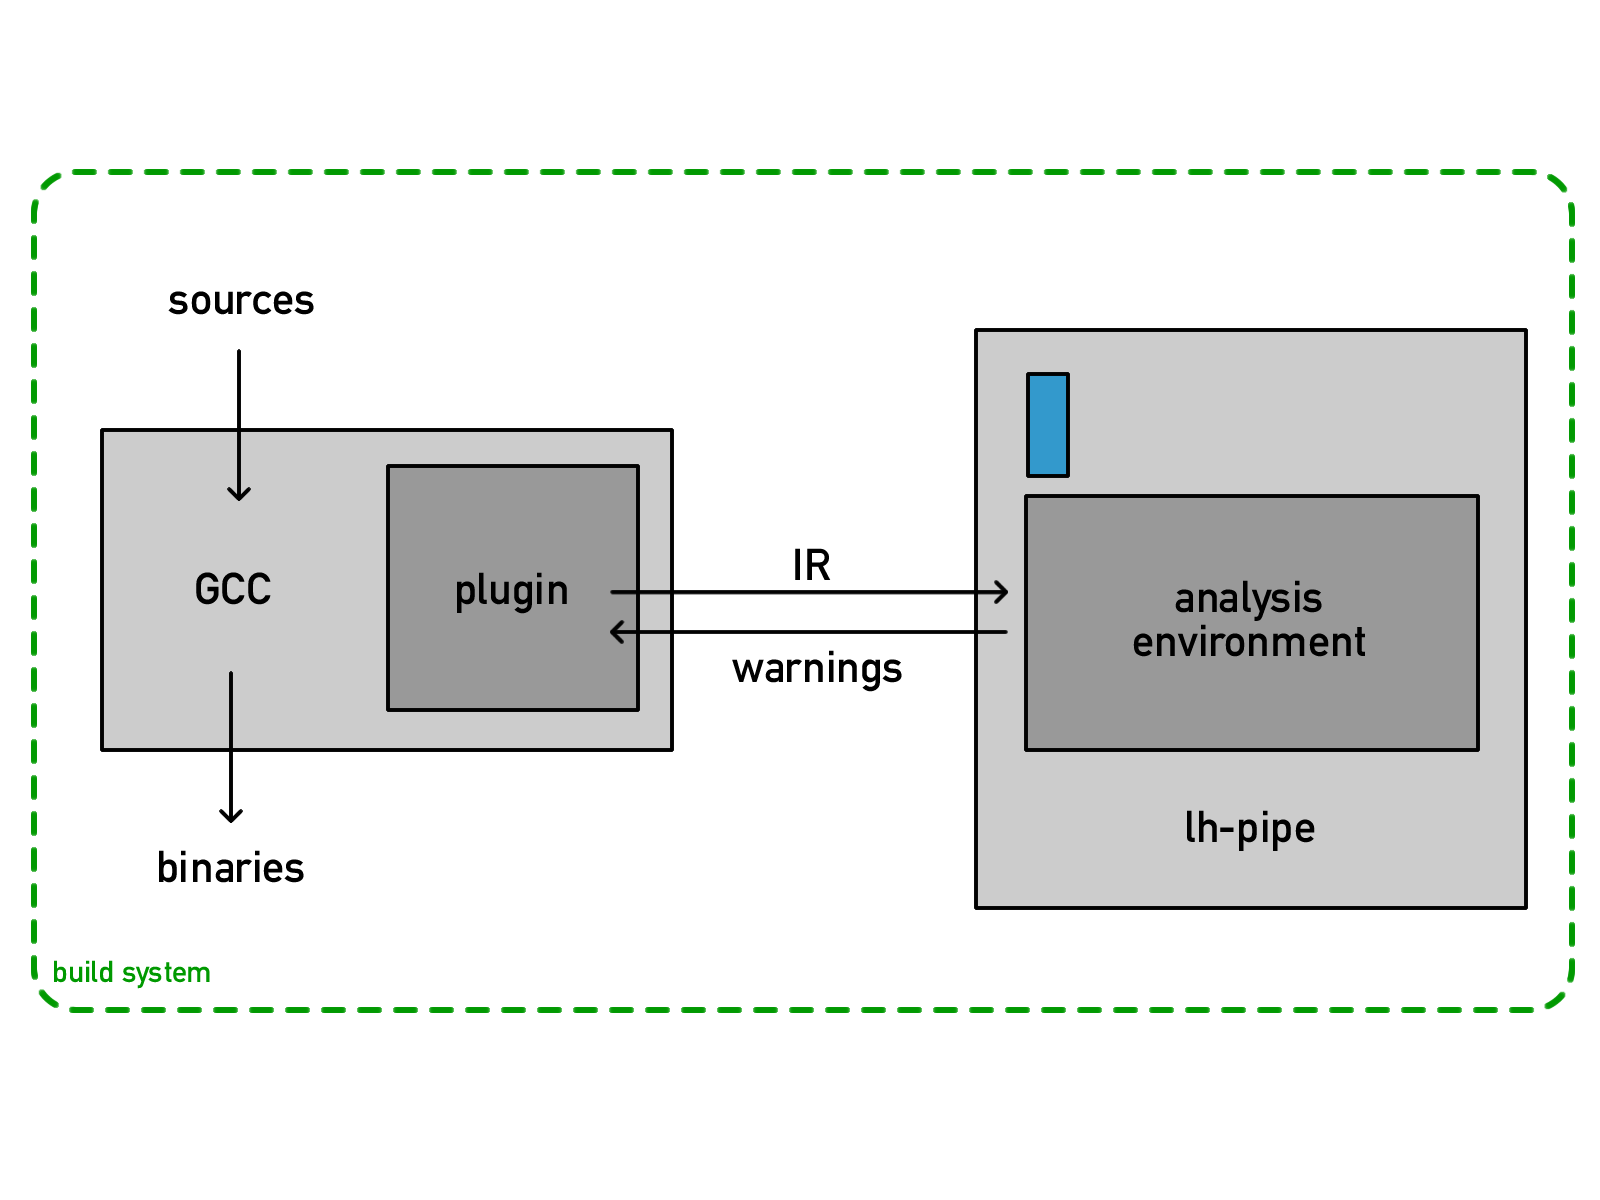
\includegraphics[width=1.0\textwidth]{arch-current.png}
}

\frame
{
  \frametitle{Results: type checking for \texttt{dsUnpackMap} et al}
  \begin{itemize}
    \item<1-> Problem: in C, arguments to \texttt{varargs}\footnote{Think \texttt{printf}, \texttt{sscanf}}
              functions cannot be type-checked by the compiler.
    \item<2-> In the oscar codebase, we have a family of such functions
              to compactly construct or deconstruct d3s messages.
  \end{itemize}
  
  \uncover<3->{Checker written in 180-odd lines of python.}
}

\begin{frame}[fragile]
  \frametitle{Results: type checking for \texttt{dsUnpackMap} et al}
\tiny \begin{verbatim}
lighthouse: Error: Value argument (index 0) to dsPackListB is not a "int"
                   as specified, but a "const unsigned int".
   call-site at: ../as_ecc.c:373:7
*** 368      DSList *poly = dsNewList(ctx->cc.a, NULL, 0);
*** 369    
*** 370      /* Run through the coefficients. */
*** 371      for (i = 0; i < D->E.field.field.poly.num_terms; i++)
*** 372      {
>>> 373        NOERR( dsPackListB(&ctx->cc, poly, "i", D->E.field.field.poly.uterms[i]) );
               ^----- call-site
*** 374      }
*** 375  
*** 376      field = dsMakeListB(ctx->cc.a, "hm", sym_AS_Binary, dsFreezeList(&poly));
*** 377    }
*** 378  
\end{verbatim}
\end{frame}

\begin{frame}[fragile]
  \frametitle{Results: type checking for \texttt{dsUnpackMap} et al}
\tiny \begin{verbatim}
lighthouse: Error: Value argument (index 2) to dsUnpackList is not a "int*"
                   as specified, but a "unsigned int*".
   call-site at: ../as_mech_hmac.c:227:21
*** 222    DSMessage *msg_hash;
*** 223    const ASMethods_CHASH *hmethods;
*** 224    unsigned int outlen;
*** 225    
*** 226    /* Our constructor is [HMAC, chash, outlen] */
>>> 227    if ( !dsUnpackList(&ctx->cc, DS_UNPACK_CHKSIZE, mech, "-mi", &msg_hash, &outlen) ||
                             ^----- call-site
*** 228         (priv->hash = asBuildMech(msg_hash, asCHASH, ctx))==NULL )
*** 229    {
*** 230      asError(sym_AS_BadMechParams, mech, ctx);
*** 231      goto x_fail;
*** 232    }
\end{verbatim}
\end{frame}

\begin{frame}[fragile]
  \frametitle{Results: type checking for \texttt{dsUnpackMap} et al}
\tiny \begin{verbatim}
lighthouse: Error: Symbol argument (index 0) to dsUnpackMap is not a DSSymbol,
                   but a "struct DSMessage**".
   call-site at: dddstest.c:2661:19
*** 2656   WANT_RC(rc, ERR_THAWED, "Check for thawed map passed on dsGetAggregateValueType");
*** 2657 
*** 2658   rc = dsGetMapKeyType(msgs[i_Map][thw], &type);
*** 2659   WANT_RC(rc, ERR_THAWED, "Check for thawed map passed on dsGetMapKeyType");
*** 2660 
>>> 2661   rc = dsUnpackMap(&ctx, DS_UNPACK_ANY, msgs[i_Map][thw], "m", &hm);
                           ^----- call-site
*** 2662   WANT_RC(rc, DS_FALSE, "Check for thawed map passed on dsUnpackMap");
*** 2663   CHK_ERR( rc, sym_Err_DSThawedError );
*** 2664 
*** 2665   CHK_RC( dsMapAdd(Map[mut], dsIncRef(str), dsIncRef(rndmsg[0])) );
*** 2666   FREEZE_DO_AND_THAW( Map, rc = OK );
\end{verbatim}
\end{frame}

\begin{frame}[fragile]
  \frametitle{Results: type checking for \texttt{dsUnpackMap} et al}
\tiny \begin{verbatim}
lighthouse: Error: Value argument (index 3) to dsUnpackMap is not a "uint8_t*"
                   as specified, but a "int8_t*".
   call-site at: dddstest.c:2502:3
*** 2497   m = dsFreezeMap(&map);
*** 2498   map = NULL;
*** 2499   FILLZERO(ctx);
*** 2500   ctx.a = a;
*** 2501   FILLZERO(uvout);
>>> 2502   CHK_OK(dsUnpackMap(&ctx, 0, m,
           ^----- call-site
*** 2503                      "v(s)v(l)v(max)v(8)v(16)v(32)v(64)",
*** 2504                      sym_Tst_First, &uvout.s,
*** 2505                      sym_Tst_Second, &uvout.l,
*** 2506                      sym_Tst_Third, &uvout.max,
*** 2507                      sym_Tst_Fourth, &uvout.u8,
\end{verbatim}
\end{frame}

\begin{frame}[fragile]
  \frametitle{Results: type checking for \texttt{dsUnpackMap} et al}
\tiny \begin{verbatim}
lighthouse: Error: Unknown format string 'U'
   call-site at: dddstest.c:2235:3
*** 2230   CHK_OK( dsPackListB(&ctx, dslist2, "v", src2.u) );
*** 2231 
*** 2232   check_equal_list(&dslist, &dslist2, "Lists created by dsPackList() differ" );
*** 2233   /* This shares code with dsPackMapMsgB(), I'm not bothering with the full invalid-format checking */
*** 2234 
>>> 2235   CHK_ERR( dsPackListB(&ctx, dslist2, "U"), sym_Err_FormatStringError );
           ^----- call-site
*** 2236 
*** 2237   /* Now unpack some lists */
*** 2238 
*** 2239   mlist = dsFreezeList(&dslist);
*** 2240 
\end{verbatim}
\end{frame}

\begin{frame}[fragile]
  \frametitle{Results: type checking for \texttt{dsUnpackMap} et al}
\tiny \begin{verbatim}
lighthouse: Warning: Call to dsUnpackMap has variable format string.
                     Verify it will always correspond with the passed in types.
   call-site at: dddstest.c:2003:9
*** 1998       case 'e': case 'E':
*** 1999       case 'u': case 'U':
*** 2000       case 'd': case 'D': break;
*** 2001 
*** 2002       case 0:
>>> 2003         CHK_OK( dsUnpackMap(&ctx, 0, m, fmt) );
                 ^----- call-site
*** 2004         break;
*** 2005 
*** 2006       default:
*** 2007         CHK_ERR( dsUnpackMap(&ctx, 0, m, fmt), sym_Err_FormatStringError );
*** 2008         break;
\end{verbatim}
\end{frame}

\begin{frame}[fragile]
  \frametitle{Results: type checking for \texttt{dsUnpackMap} et al}
\tiny \begin{verbatim}
lighthouse: Error: Value argument (index 0) to dsUnpackMap is not a "uint32_t*"
                   as specified, but a "ntl_connection_t*".
   call-site at: ../ntl_remote.c:1143:20
*** 1138 
*** 1139   FILLZERO(ctx);
*** 1140   ctx->a = inst->xa;
*** 1141   NTL_MUTEX_ACQUIRE(ntl__remote_mutex); locked = 1; {
*** 1142     /* Extract the connection handle */
>>> 1143     if(!dsUnpackMap(ctx, 0, reply, "v(32)",
                            ^----- call-site
*** 1144                     sym_NTL_RPC_CONNECTION, conn_out)) {
*** 1145       D(("dsUnpackMap failed"));
*** 1146       status = NTL_ERROR_RPC_PROTOCOL;
*** 1147       goto error;
*** 1148     }
\end{verbatim}
\end{frame}

\frame
{
  \frametitle{Results: build performance}

  A full \texttt{buildme} in \texttt{nglibs} took:
  
  \begin{description}
    \item<2->[119 CPU seconds] Without plugin loaded.
    \item<3->[134 CPU seconds] With plugin loaded.
  \end{description}
}

\frame
{
  \frametitle{Things for the future}

  \begin{itemize}
    \item<1-> Write checker for \texttt{PyArg\_ParseTuple()} et al and compile
              lots of python extensions.
    \item<2-> Write proper data flow analysis tools for use by checkers, so they can do
              analysis of resource lifetimes, etc.
    \item<3-> Build out separate analysis system so we can do proper inter-procedural
              analysis.
  \end{itemize}
}

\frame
{
  \frametitle{Fin}
  Questions?
}

\end{document}
